\documentclass[conference]{IEEEtran}
\IEEEoverridecommandlockouts
\usepackage{amsmath,amssymb,amsfonts}
\usepackage{algorithm}
\usepackage{algpseudocode}
\usepackage{graphicx}
\usepackage{booktabs}
\usepackage{multirow}
\usepackage[table]{xcolor}
\usepackage{tikz}
\usetikzlibrary{positioning,arrows.meta,fit,backgrounds}
\usepackage[hidelinks]{hyperref}

\newcommand{\R}{\mathbb{R}}
\newcommand{\hs}{\hat{s}}
\DeclareMathOperator*{\argmax}{arg\,max}

\begin{document}

\title{OCD-Mix: Multi-Scale Online Change-Point Detection and Quantification for High-Dimensional Temporally Dependent Streams}

\author{\IEEEauthorblockN{Keshav Sharma}
\IEEEauthorblockA{[Affiliation, city, country]\\ [email]}
\and
\IEEEauthorblockN{Shivam Singh}
\IEEEauthorblockA{[Affiliation, city, country]\\ [email]}}

\maketitle

\begin{abstract}
Online change-point detectors for high-dimensional streams are usually calibrated for independent observations. When the streams are serially correlated, window sums vary far more than such detectors expect, and false alarms follow. We present OCD-Mix, an online multi-scale detector of persistent sparse or dense mean shifts in serially dependent high-dimensional streams, with post-alarm quantification. OCD-Mix standardises dyadic-window sums with prewhitened long-run variance estimates taken from a change-free training segment, corrects them for finite windows and for the estimated baseline mean, and monitors a maximum chart for sparse shifts and a quadratic chart for dense ones. Thresholds are calibrated by simulation, either from an archive of null streams or from the stream's own training data. After an alarm, OCD-Mix localises the change, reports the affected coordinates and builds a confidence interval by adapting the Chen--Wang--Samworth procedure. On a diagonal VAR(1) benchmark with $p=50$, an independence-based detector of the same family alarmed on every null stream for $\phi\ge 0.3$. With archive-calibrated thresholds, OCD-Mix had false-alarm rates of 4.6--5.6\% on 2000 held-out null streams per dependence level (target 5\%); autonomous self-calibration gave 7.1--9.8\%. On 1000 held-out change streams per cell, OCD-Mix detected 98.1--98.8\% of changes, and its intervals covered the true change point in 96.2--98.5\% of detections. On identical streams, CWS, RFF-MMD and NEWMA calibrated under independence alarmed on every null stream for $\phi\ge 0.3$; even with oracle thresholds tuned at the true $\phi$ they needed 10--50\% more steps to detect than OCD-Mix. Monitoring costs $O(p|\mathcal{K}|)$ time per observation and $O(pk_{\max})$ memory. Guarantees under estimated parameters are not established, and under dense non-diagonal dynamics the false-alarm rate rises to 30.5\%.
\end{abstract}

\begin{IEEEkeywords}
online change-point detection, data streams, high-dimensional time series, long-run variance, temporal dependence, post-alarm inference
\end{IEEEkeywords}

\section{Introduction}
Cloud telemetry, sensor arrays, network counters and industrial monitors produce continuous high-dimensional streams whose behaviour changes abruptly when hardware degrades, a link fails, a sensor is recalibrated or a workload moves. Reliable stream processing needs to flag such a change quickly, keep false alarms rare, and say \emph{when} the change happened and \emph{which} dimensions it touched. Early data-management work treated stream change detection as a comparison of windows under independence~\cite{kifer2004}; more recent work segments streams efficiently~\cite{ermshaus2024}.

\textbf{Temporal dependence breaks independence-based detectors.} Online detectors with strong guarantees, such as the multiscale procedure of Chen, Wang and Samworth~\cite{chen2022}, assume independent Gaussian observations. Real streams are autocorrelated: queues, inertia and feedback make consecutive measurements alike. For a coordinate with lag-one autocorrelation $\phi$, the variance of a long window sum is inflated by about $(1+\phi)/(1-\phi)$ relative to the independent case, so a detector that standardises by the marginal variance sees inflated statistics. In our benchmark, an independence-based detector alarmed on every null stream, on average after 224 steps at $\phi=0.3$ and after 8 steps at $\phi=0.8$ (Sec.~\ref{sec:far}).

\textbf{Why quantification matters.} An alarm alone is rarely actionable. Operators need the change location, a confidence interval for it and the affected dimensions. Chen et al.~\cite{chen2024} showed how to deliver an interval with nominal coverage and a support estimate online, but only under independence.

\textbf{Gap.} Online high-dimensional detectors with post-alarm inference were developed for independent data~\cite{chen2024,chen2022,mei2010,xie2013}. Methods for dependent series are offline~\cite{padilla2023}, low-dimensional or self-normalised~\cite{shao2010}, or make minimal assumptions at the price of power in structured settings~\cite{shekhar2024}. We know of no detector that combines dependence-aware standardisation, sparse and dense charts, bounded-memory monitoring and coordinate-level post-alarm inference.

\textbf{OCD-Mix.} OCD-Mix (i) estimates per-coordinate long-run variances (LRVs) by AR(1) prewhitening of a change-free training segment, (ii) turns them into a finite-window normalisation that accounts for baseline-mean uncertainty, (iii) monitors dyadic windows from cumulative-sum ring buffers with a maximum chart and a quadratic chart, (iv) calibrates thresholds by simulation, optionally from the stream's own training data, and (v) after an alarm localises the change, recovers the affected coordinates and builds an interval, adapting~\cite{chen2024} to LRV-standardised dependent data. Bounded per-observation cost and memory that does not grow with the stream come from the multiscale design of~\cite{chen2022}; our contribution is to make that design work under serial dependence and to measure where it does and does not.

\textbf{Scope.} OCD-Mix targets \emph{persistent mean shifts}. It is not a point- or subsequence-anomaly detector~\cite{schmidl2022,tuli2022}, nor a concept-drift detector for model error or arbitrary distributional change~\cite{gama2014,lu2019}. Its validated dependence class is \emph{diagonal} VAR(1); we do not claim robustness to arbitrary $\alpha$-mixing processes.

\textbf{Contributions.}
\begin{enumerate}
\item A dependence-aware standardisation for multiscale online monitoring: prewhitened Bartlett LRVs combined with a finite-window variance table and a baseline-mean term. The empirical second moment of the standardised window sums stayed in $[1.005,1.057]$ across scales 8--512 and $\phi\in[0,0.8]$ (Sec.~\ref{sec:method}).
\item A dual-chart detector (maximum and unthresholded quadratic) with two simulation-based calibration modes, one of them autonomous. Both are evaluated on held-out null streams, and we report explicitly how much false-alarm inflation parameter estimation causes (Secs.~\ref{sec:calib},~\ref{sec:far}).
\item An adaptation of post-alarm localisation, support recovery and confidence-interval construction to LRV-standardised dependent data, with held-out coverage of 96.2--98.5\% against a 95\% target. It replaces an earlier heuristic interval that under-covered (83.8\% at $\phi=0$) (Secs.~\ref{sec:support},~\ref{sec:ci}).
\item A streaming cost analysis and a frank account of limits: $O(p|\mathcal{K}|)$ monitoring time, $O(pk_{\max})$ memory, 117--136\,$\mu$s per update for $p\le 400$, a side-by-side comparison with published detectors on the same streams, and a documented failure mode under dense non-diagonal dynamics (false-alarm rate up to 30.5\%) (Secs.~\ref{sec:complexity},~\ref{sec:exp}).
\end{enumerate}
The individual components are classical. What we contribute is their integration, calibration and evaluation for dependent streams, not a new robustness theorem.

\section{Related Work}
\subsection{Online and sequential change detection}
Sequential change detection began with CUSUM~\cite{page1954} and its optimality theory~\cite{lorden1971}. For many streams, Mei~\cite{mei2010} sums local CUSUM statistics, and Xie and Siegmund~\cite{xie2013} use a mixture that soft-thresholds local statistics for sparse changes; both treat the streams as independent. Chen, Wang and Samworth~\cite{chen2022} give a multiscale procedure for high-dimensional Gaussian mean changes, with patience guarantees and sparsity-dependent delay bounds, whose storage and per-observation cost do not depend on the number of past observations. OCD-Mix keeps this bounded-state architecture. Kalinke and Gavioli-Akilagun~\cite{kalinke2025} give a non-parametric kernel detector based on random Fourier features (RFF-MMD) with logarithmic time and space, minimax-optimal delay and no need for pre-change training data, again for independent observations. Shekhar and Ramdas~\cite{shekhar2024} reduce detection to sequential estimation with confidence sequences and obtain an average run length of at least $1/\alpha$ under minimal assumptions; applying their reduction to high-dimensional dependent streams requires a valid confidence sequence for a dependent mean, which is exactly the difficulty we address parametrically.

\subsection{High-dimensional detection and inference}
Offline theory characterises sparse high-dimensional mean-change detection through minimax rates~\cite{liu2021}, sparse alternatives~\cite{enikeeva2019}, and localisation by sparse projection~\cite{wang2018} or sparsified binary segmentation~\cite{cho2015}. Online uncertainty quantification was missing until Chen et al.~\cite{chen2024}, who give a confidence interval with nominal coverage and length of the order of the detection delay (up to a logarithmic factor), plus a support estimate, for any base detector meeting patience and delay conditions. OCD-Mix adopts this inference machinery but runs it on LRV-standardised statistics from a different base detector, so their coverage theorem does not apply directly (Sec.~\ref{sec:ci}).

\subsection{Change detection under temporal dependence}
Standardising sums of dependent data needs a long-run variance. Kernel HAC estimators~\cite{newey1987,andrews1991} are biased downward under strong autocorrelation; prewhitening reduces the bias but can increase variance~\cite{andrews1992}. Both effects show up here: Sec.~\ref{sec:exp} reports the bias reduction and a residual false-alarm excess consistent with estimation variance. Dependent-data methods include self-normalised tests~\cite{shao2010}, sequential monitoring of time-series parameters that avoids LRV estimation~\cite{dette2020}, and offline multivariate non-parametric localisation under exponentially decaying $\alpha$-mixing with a block-type LRV estimator~\cite{padilla2023}. Their guarantees do not transfer to our setting because they are offline, low-dimensional, or provide no coordinate-level post-alarm inference. OCD-Mix is parametric in the dependence (per-coordinate AR(1) prewhitening), hence narrower in scope, but supports bounded-memory high-dimensional monitoring with attribution.

\subsection{Streaming analytics and data engineering}
Kifer et al.~\cite{kifer2004} compare sliding windows with distribution-free statistics under independence. ClaSS~\cite{ermshaus2024} segments streams by self-supervised classification, at a cost linear in the window size, and ships as a Flink operator. Time-series anomaly detection looks for points or subsequences that deviate from a model~\cite{schmidl2022}, increasingly with learned reconstruction models~\cite{tuli2022}, and concept-drift detection targets changes that hurt a learner~\cite{gama2014,lu2019}. These tasks differ from persistent mean-shift detection: anomalies may be transient, drift is defined relative to a model, and none of them gives a calibrated alarm rule together with a confidence interval for the change time and a set of affected coordinates.

\section{Preliminaries and Problem Formulation}
Let $X_t\in\R^p$, $t=1,2,\dots$, arrive sequentially. We consider a single persistent mean change,
\begin{equation}
X_t=\mu+\theta\,\mathbb{1}\{t>z\}+Z_t, \label{eq:model}
\end{equation}
where $\mu\in\R^p$ is the unknown pre-change mean, $\theta\in\R^p\setminus\{0\}$ the change, $z\in\{m_0,m_0+1,\dots\}\cup\{\infty\}$ the unknown change time ($z=\infty$ is a null stream), and $(Z_t)$ a zero-mean, strictly stationary noise process with finite second moments. The support is $S=\{j:\theta_j\neq 0\}$ with $s=|S|$; $s\ll p$ is the sparse and $s\asymp p$ the dense regime. Table~\ref{tab:notation} lists the main symbols.

\begin{table}[t]
\centering
\caption{Main notation.}
\label{tab:notation}
\small
\begin{tabular}{@{}ll@{}}
\toprule
Symbol & Meaning\\
\midrule
$p,T,m_0$ & dimension, stream length, training length\\
$z,\theta,S,s$ & change time, shift, support, sparsity\\
$\hat\mu_j,\hat\gamma_{0,j},\hat r_j$ & training mean, variance, clipped AR(1) coefficient\\
$\hat\omega_j,\hat\sigma^2_j$ & innovation LRV, prewhitened LRV\\
$\hat v_{k,j},\hs^2_{k,j}$ & finite-window variance rate, window variance\\
$\mathcal{K}=\{k_{\min}2^{i-1}\}$ & dyadic window grid ($8,\dots,512$)\\
$W_{t,k,j}$ & standardised window sum\\
$A_{t,k},Q_{t,k}$ & maximum and quadratic charts\\
$\tau_A,\tau_Q,c_A,c_Q$ & thresholds and calibrated multipliers\\
$N,t_N$ & alarm time, largest violating scale\\
$m^*,\hat\nu$ & localised window length, change estimate\\
$\hat\jmath,\hat S,\hat S_{\mathrm{rep}}$ & anchor, CI support, reported support\\
$\tilde b_j,t_j$ & signed signal scale, CUSUM tail length\\
\bottomrule
\end{tabular}
\end{table}

\textbf{Timeline.} Observations $1,\dots,m_0$ form a change-free \emph{training} segment ($z>m_0$) from which all baseline parameters are estimated; monitoring runs for $t>m_0$ up to the horizon $H=T-m_0$ ($T=5000$, $m_0=1000$, $H=4000$ in our experiments).

\textbf{Dependence.} Our benchmark generates $Z_t=AZ_{t-1}+\varepsilon_t$ with $\varepsilon_t\overset{\text{i.i.d.}}{\sim}N_p(0,\Sigma_\varepsilon)$ and $\|A\|_2<1$, a stable Gaussian VAR(1), which is geometrically strongly mixing; we use this only to motivate the model class. The method models each coordinate as a univariate AR(1), $Z_{t,j}=r_jZ_{t-1,j}+e_{t,j}$ with $|r_j|\le 0.95$. This is exact in the validated case $A=\phi I_p$, $\phi\in\{0,0.3,0.6,0.8\}$, and an approximation otherwise; \emph{validity is established empirically only for diagonal $A$}.

\textbf{Objectives.} (i) False-alarm probability: $P_\infty(N\le m_0+H)\le\alpha_0$ with $\alpha_0=0.05$; this is a calibration target, not a proven bound under estimated parameters. (ii) Detection delay $E_z[N-z\mid N>z]$. (iii) Localisation error $|\hat\nu-z|$. (iv) Interval coverage $P_z(z\in\mathrm{CI}\mid N\ge z)\ge 1-\alpha$, $\alpha=0.05$. (v) Support recovery measured by the Jaccard index $J(\hat S_{\mathrm{rep}},S)=|\hat S_{\mathrm{rep}}\cap S|/|\hat S_{\mathrm{rep}}\cup S|$. (vi) Per-observation time and memory independent of stream length.

\section{The OCD-Mix Framework}
Fig.~\ref{fig:arch} shows the architecture. An \emph{offline stage} uses only the training segment: it estimates per-coordinate dependence, LRVs and the finite-window normalisation table, and calibrates thresholds by simulating null streams (from an archive or from a model fitted to the stream itself). An \emph{online stage} then ingests one vector at a time, updates cumulative-sum ring buffers, evaluates both charts at every dyadic scale and stops at the first threshold crossing. A \emph{post-alarm stage} runs once on the buffered recent history. The separation matters for resources: training and calibration are one-off costs, monitoring is the per-observation bottleneck, and post-alarm inference is off the critical path. The detector never sees ground truth; a unit test checks that detection and calibration modules never read change-point labels.

\begin{figure*}[t]
\centering
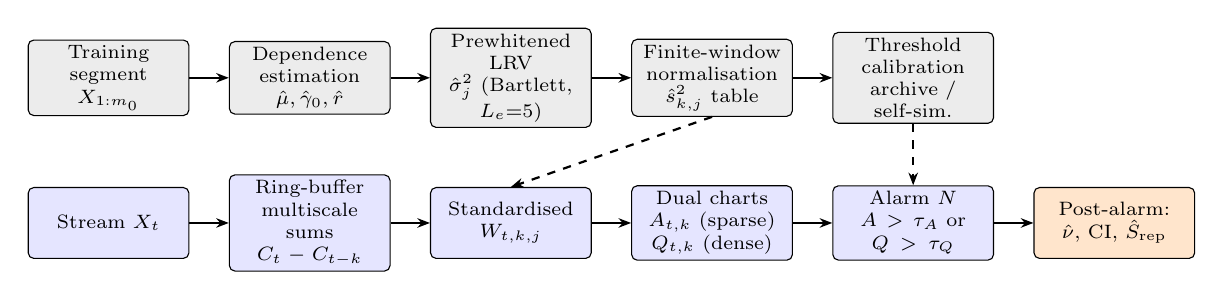
\begin{tikzpicture}[node distance=4mm and 5mm, font=\scriptsize,
 box/.style={draw, rounded corners=2pt, align=center, minimum height=9mm, inner sep=2pt, text width=19mm},
 off/.style={box, fill=gray!15}, on/.style={box, fill=blue!10}, post/.style={box, fill=orange!20},
 arr/.style={-{Stealth[length=1.6mm]}, thick}]
\node[off] (tr) {Training segment\\$X_{1:m_0}$};
\node[off, right=of tr] (dep) {Dependence\\estimation\\$\hat\mu,\hat\gamma_0,\hat r$};
\node[off, right=of dep] (lrv) {Prewhitened LRV\\$\hat\sigma_j^2$ (Bartlett, $L_e{=}5$)};
\node[off, right=of lrv] (fw) {Finite-window\\normalisation\\$\hs^2_{k,j}$ table};
\node[off, right=of fw] (cal) {Threshold\\calibration\\archive / self-sim.};
\node[on, below=9mm of tr] (st) {Stream $X_t$};
\node[on, right=of st] (rb) {Ring-buffer\\multiscale sums\\$C_t-C_{t-k}$};
\node[on, right=of rb] (w) {Standardised\\$W_{t,k,j}$};
\node[on, right=of w] (ch) {Dual charts\\$A_{t,k}$ (sparse)\\$Q_{t,k}$ (dense)};
\node[on, right=of ch] (al) {Alarm $N$\\$A>\tau_A$ or $Q>\tau_Q$};
\node[post, right=of al] (pa) {Post-alarm:\\$\hat\nu$, CI, $\hat S_{\mathrm{rep}}$};
\draw[arr] (tr)--(dep); \draw[arr] (dep)--(lrv); \draw[arr] (lrv)--(fw); \draw[arr] (fw)--(cal);
\draw[arr] (st)--(rb); \draw[arr] (rb)--(w); \draw[arr] (w)--(ch); \draw[arr] (ch)--(al); \draw[arr] (al)--(pa);
\draw[arr, dashed] (fw.south)--(w.north); \draw[arr, dashed] (cal.south)--(al.north);
\end{tikzpicture}
\caption{OCD-Mix architecture. Grey: one-off offline stage on the change-free training segment; blue: online monitoring with $O(p|\mathcal{K}|)$ time and $O(pk_{\max})$ memory per update; orange: post-alarm inference, executed once.}
\label{fig:arch}
\end{figure*}

\section{Methodology}\label{sec:method}
\subsection{Training and baseline estimation}
For each coordinate $j\in[p]$ the training segment gives
\begin{align}
\hat\mu_j&=\tfrac{1}{m_0}\textstyle\sum_{t=1}^{m_0}X_{t,j},\qquad X^c_{t,j}=X_{t,j}-\hat\mu_j, \label{eq:mu}\\
\hat\gamma_{0,j}&=\tfrac{1}{m_0}\textstyle\sum_{t=1}^{m_0}(X^c_{t,j})^2, \label{eq:g0}\\
\hat r_j&=\mathrm{clip}\Big(\frac{\sum_{t=2}^{m_0}X^c_{t-1,j}X^c_{t,j}}{\sum_{t=2}^{m_0}(X^c_{t-1,j})^2},-0.95,0.95\Big). \label{eq:r}
\end{align}
Equations~\eqref{eq:mu}--\eqref{eq:g0} are the sample mean and marginal variance, and \eqref{eq:r} is the least-squares lag-one coefficient. Clipping to $[-0.95,0.95]$ keeps the factor $(1-\hat r_j)^{-2}$ from exploding as $\hat r_j\to 1$. All estimates require a change-free training segment; contamination would bias $\hat\mu$ and inflate the variances.

\subsection{Prewhitened long-run variance}
The LRV $\sigma_j^2=\sum_{h\in\mathbb{Z}}\gamma_j(h)$ governs long window sums: $\mathrm{Var}(\sum_{i\le k}Z_{i,j})\approx k\sigma_j^2$. A direct Bartlett estimate truncates the autocovariance sum and is strongly biased downward under high autocorrelation (in our tests $-4.9\%$, $-10.8\%$ and $-22.9\%$ at $\phi=0.3,0.6,0.8$ with $L=20$). Following Andrews and Monahan~\cite{andrews1992}, we first filter out the dominant serial dependence. The residuals and their recentred versions are
\begin{equation}
\hat e_{t,j}=X^c_{t,j}-\hat r_jX^c_{t-1,j},\qquad \tilde e_{t,j}=\hat e_{t,j}-\tfrac{1}{m_0-1}\textstyle\sum_{s=2}^{m_0}\hat e_{s,j}, \label{eq:resid}
\end{equation}
for $t=2,\dots,m_0$. These are close to white, so a short-bandwidth Bartlett estimator suffices:
\begin{equation}
\hat\omega_j=\tilde\gamma_{e,j}(0)+2\sum_{h=1}^{L_e}\Big(1-\frac{h}{L_e+1}\Big)\tilde\gamma_{e,j}(h), \label{eq:omega}
\end{equation}
with $\tilde\gamma_{e,j}(h)=\frac{1}{m_0-1}\sum_{t=2}^{m_0-h}\tilde e_{t,j}\tilde e_{t+h,j}$, $L_e=5$, floored at $10^{-8}$. Recolouring through the AR(1) transfer function at frequency zero, $f_X(0)=f_e(0)/(1-r)^2$, gives
\begin{equation}
\hat\sigma_j^2=\hat\omega_j/(1-\hat r_j)^2. \label{eq:sigma}
\end{equation}
With $m_0=1000$ the bias of \eqref{eq:sigma} was $-0.21\%$, $-0.07\%$ and $+0.02\%$ at $\phi=0.3,0.6,0.8$, more than an order of magnitude below the direct estimate. The scalar AR(1) filter is exact for diagonal dynamics; under cross-coupling it removes only each coordinate's marginal serial dependence (Sec.~\ref{sec:limits}). As in~\cite{andrews1992}, lower bias comes at the price of higher estimator variance, which we later see as false-alarm inflation under self-calibration.

\subsection{Finite-window variance normalisation}
Normalising a window sum by $k\hat\sigma_j^2$ is inaccurate for short windows, and centring by $\hat\mu_j$ adds variance. For a stationary AR(1) with autocovariance $\gamma_0r^{|h|}$, summing the autocovariances over a window of length $k$ gives
\begin{equation}
\frac1k\mathrm{Var}\Big(\sum_{i=1}^kY_i\Big)=\sigma^2-\frac{2\gamma_0r(1-r^k)}{k(1-r)^2},\qquad \sigma^2=\gamma_0\frac{1+r}{1-r}. \label{eq:fw}
\end{equation}
OCD-Mix uses the plug-in version with the prewhitened $\hat\sigma_j^2$ in place of $\sigma^2$ and a floor for stability,
\begin{equation}
\hat v_{k,j}=\max\Big(\hat\sigma_j^2-\frac{2\hat\gamma_{0,j}\hat r_j(1-\hat r_j^k)}{k(1-\hat r_j)^2},\;0.2\,\hat\gamma_{0,j}\Big). \label{eq:v}
\end{equation}
Identity~\eqref{eq:fw} is exact for AR(1) autocovariances with known parameters; \eqref{eq:v} is an approximation because $\hat\sigma^2_j$ comes from a different (prewhitened) route and need not equal $\hat\gamma_{0,j}(1+\hat r_j)/(1-\hat r_j)$. The centred window sum $\sum_i(X_{i,j}-\hat\mu_j)=S_k-\frac{k}{m_0}S^{\mathrm{train}}_{m_0}$ then has variance approximately
\begin{equation}
\hs^2_{k,j}=k\hat v_{k,j}+\frac{k^2\hat\sigma_j^2}{m_0}. \label{eq:s2}
\end{equation}
This treats the monitoring and training blocks as uncorrelated and uses $\mathrm{Var}(S^{\mathrm{train}}_{m_0})\approx m_0\sigma_j^2$. Both are approximations: the cross-covariance is negligible only when the blocks are separated by more than the dependence range. We therefore regard \eqref{eq:s2} as a validated approximation, not an identity. The table $\hs^2_{m,j}$ is computed for all integers $m\le 2k_{\max}$. Empirically, $E[W^2_{t,k,j}]$ stayed in $[1.005,1.057]$ over $k\in\{8,32,128,512\}$ and $\phi\in\{0,0.3,0.6,0.8\}$ (20 null streams), inside the acceptance range $[0.93,1.10]$.

\subsection{Online multiscale monitoring}
The dyadic grid $\mathcal{K}=\{k_{\min}2^{i-1}\}_{i=1}^7=\{8,16,\dots,512\}$ spans almost three orders of magnitude with seven scales: for any delay $\Delta\in[k_{\min},2k_{\max})$ some $k\in\mathcal{K}$ satisfies $k\le\Delta<2k$, so a window at most twice the ideal length is always available. Windows lie entirely in the monitoring period, $t-k\ge m_0$. With centred observations $x_t=X_t-\hat\mu$, the running sum
\begin{equation}
C_{t,j}=\sum_{u=m_0}^t x_{u,j},\qquad \sum_{i=t-k+1}^t x_{i,j}=C_{t,j}-C_{t-k,j} \label{eq:cusum}
\end{equation}
yields any window sum with one vector subtraction, so a circular buffer of the last $k_{\max}+1$ values of $C_t$ suffices. To avoid floating-point cancellation on very long streams, the buffer is re-anchored every $k_{\max}$ steps by subtracting its oldest entry (the offset is stored separately). A second circular buffer keeps the last $2k_{\max}$ centred observations for post-alarm analysis. The streaming detector reproduced the batch statistics to relative tolerance $10^{-9}$.

\subsection{Dual-chart detection statistics}
The standardised window sum is
\begin{equation}
W_{t,k,j}=\frac{1}{\hs_{k,j}}\sum_{i=t-k+1}^{t}(X_{i,j}-\hat\mu_j), \label{eq:W}
\end{equation}
approximately $N(0,1)$ per coordinate under the null. Two charts summarise $W_{t,k}\in\R^p$:
\begin{equation}
A_{t,k}=\max_{j\in[p]}|W_{t,k,j}|,\qquad Q_{t,k}=\frac{\sum_{j=1}^pW_{t,k,j}^2-p}{\sqrt{2p}}. \label{eq:charts}
\end{equation}
Chart $A$ is sensitive to sparse shifts: one strongly shifted coordinate stands out and unaffected coordinates add no noise. Chart $Q$ pools weak shifts across many coordinates and responds to dense shifts; unlike the thresholded quadratic chart of~\cite{chen2022}, it has no coordinate threshold to tune. We do not assume $Q$ is standard normal. If every $W_{t,k,j}$ has unit variance, $E[\sum_jW_j^2]=p$ whatever the cross-coordinate correlation, so $E[Q]=0$; but for jointly Gaussian $W$ with correlation matrix $R$, $\mathrm{Var}(\sum_jW_j^2)=2\|R\|_F^2$, hence
\begin{equation}
\mathrm{Var}(Q_{t,k})=\|R\|_F^2/p\ \ge\ 1, \label{eq:varQ}
\end{equation}
with equality only for $R=I_p$. Spatial dependence therefore changes the spread and tail of $Q$, not its mean, which is why $\tau_Q$ is calibrated by simulation rather than taken from a normal approximation.

\subsection{Null distribution and threshold calibration}\label{sec:calib}
Let $M_A=\max_{t>m_0,k\in\mathcal{K}}A_{t,k}/\sqrt{2\ln(2p|\mathcal{K}|)}$ and $M_Q=\max_{t>m_0,k\in\mathcal{K}}Q_{t,k}$ be the null maxima over the horizon. The thresholds are
\begin{equation}
\tau_A=c_A\sqrt{2\ln(2p|\mathcal{K}|)},\qquad \tau_Q=c_Q, \label{eq:tau}
\end{equation}
where the Gaussian extreme-value scale gives $c_A$ an interpretable magnitude and $c_A,c_Q$ absorb temporal and spatial dependence.

\textbf{Archive calibration.} Given $n_{\mathrm{sim}}$ null streams, fitted and monitored exactly like a real stream, we split $\alpha_0=0.05$ between the charts (Bonferroni):
\begin{equation}
c_A=\mathrm{Quantile}_{1-\alpha_0/2}(\{M_{A,i}\}),\quad c_Q=\mathrm{Quantile}_{1-\alpha_0/2}(\{M_{Q,i}\}). \label{eq:calib}
\end{equation}
By the union bound this controls the probability that either chart crosses within the horizon at $\alpha_0$ under the simulated law, up to Monte Carlo error. The thresholds used throughout Sec.~\ref{sec:exp} were calibrated on $n_{\mathrm{sim}}=4000$ null streams per dependence level, generated at the dependence level of the evaluation streams. A joint variant (marginal quantiles followed by a common rescaling) differed by less than 2.3\%.

\textbf{Autonomous self-calibration.} When no archive exists, the detector fits $\hat r$ and the innovation covariance $\hat\Sigma_\varepsilon=\frac{1}{m_0-1}\sum_t\tilde e_t\tilde e_t^\top$ from its own training segment, symmetrises and regularises it, forms $\hat\Gamma_{0,ij}=\hat\Sigma_{\varepsilon,ij}/(1-\hat r_i\hat r_j)$, simulates $n_{\mathrm{sim}}=300$ null streams of length $T$ via $Z_0\sim N(0,\hat\Gamma_0)$, $Z_t=\hat r\odot Z_{t-1}+\varepsilon_t$, $\varepsilon_t\sim N(0,\hat\Sigma_\varepsilon)$, and applies~\eqref{eq:calib}. This parametric bootstrap inherits the estimation error of $\hat r$ and $\hat\Sigma_\varepsilon$, so we report its false-alarm rate only on fresh out-of-sample null streams (Sec.~\ref{sec:far}).

\subsection{Sequential alarm generation}
Monitoring stops at
\begin{equation}
N=\inf\{t>m_0:\exists k\in\mathcal{K},\ A_{t,k}>\tau_A\ \text{or}\ Q_{t,k}>\tau_Q\}, \label{eq:N}
\end{equation}
so a crossing of either chart at any scale raises the alarm. Several scales may exceed their thresholds at $N$; the largest,
\begin{equation}
t_N=\max\{k\in\mathcal{K}:A_{N,k}>\tau_A\ \text{or}\ Q_{N,k}>\tau_Q\}, \label{eq:tN}
\end{equation}
reaches furthest back and is the best dyadic indication of the change's age. It bounds the post-alarm search and sets the window used for support recovery and the interval.

\subsection{Post-alarm change-point localisation}
Because the dyadic grid restricts window lengths to powers of two, after an alarm OCD-Mix scans every integer length $m\in[k_{\min},\min(2t_N,N-m_0+1)]$ on the buffered observations and picks
\begin{equation}
m^*=\argmax_m\max\Big(\frac{A_{N,m}}{\tau_A},\frac{Q_{N,m}}{\tau_Q}\Big),\qquad \hat\nu=N-m^*+1, \label{eq:mstar}
\end{equation}
where $A_{N,m},Q_{N,m}$ use the table entry $\hs^2_{m,j}$. The criterion picks the window length at which the stronger chart is most extreme relative to its threshold, and the change is placed at its left end. With cumulative sums the scan costs $O(pk_{\max})$.

\subsection{Coordinate support recovery}\label{sec:support}
The anchor is the coordinate with the strongest response at the alarm scale, $\hat\jmath=\argmax_{j}|W_{N,t_N,j}|$. Because $\hat\jmath$ is selected by the stopping rule, it is treated apart from the other coordinates. With $\ell\ge 0$ extra post-alarm observations ($\ell=0$ by default) and $k=t_N+\ell$, define $E_j=\hs_{k,j}^{-1}\sum_{i=N-t_N+1}^{N+\ell}(X_{i,j}-\hat\mu_j)$ and $d_{1,c}=c\sqrt{\log(p/\alpha)}$. Two support sets use two constants:
\begin{align}
\hat S&=\{j\neq\hat\jmath:\ |E_j|-b_{\min}\sqrt{k}\ge d_{1,\mathrm{CI}}\}, \label{eq:S}\\
\hat S_{\mathrm{rep}}&=\{j\neq\hat\jmath:\ |E_j|-b_{\min}\sqrt{k}\ge d_{1,\mathrm{rep}}\}\cup\{\hat\jmath\}. \label{eq:Srep}
\end{align}
$\hat S$ (anchor excluded, lower threshold) feeds the interval; $\hat S_{\mathrm{rep}}$ (higher threshold, anchor always included) is what the user sees and what the Jaccard index scores. We use $c_{\mathrm{CI}}=0.40$, $c_{\mathrm{rep}}=0.80$ and $b_{\min}=0.1$; the constants were tuned on dedicated calibration seeds, not derived from theory.

\subsection{Post-alarm confidence interval}\label{sec:ci}
We adapt the interval of Chen et al.~\cite{chen2024}. A dyadic grid of standardised amplitudes is $B_0=\{b_{\min}\}$, $B=\{2^{m/2}b_{\min}:m=1,\dots,\lceil 2\log_2(1/b_{\min})\rceil\}$. For $j\in\hat S$ the signed signal-scale estimate is
\begin{equation}
\tilde b_j=\mathrm{sgn}(E_j)\max\{b\in B\cup B_0:\ |E_j|-b\sqrt{k}\ge d_{1,\mathrm{CI}}\}. \label{eq:btilde}
\end{equation}
With $\zeta_{i,j}=(X_{i,j}-\hat\mu_j)/\hat\sigma_j$, the backward CUSUM tail length is
\begin{equation}
t_j=\text{smallest}\argmax_{0\le h\le h_{\max}}\Big[\tilde b_j\sum_{i=N-h+1}^{N}\Big(\zeta_{i,j}-\frac{\tilde b_j}{2}\Big)\Big], \label{eq:tj}
\end{equation}
with ties broken towards the smallest $h$ to avoid artificial expansion on flat objectives, and the interval is
\begin{equation}
\mathrm{CI}=\Big[\max\Big(m_0,\ N-\min_{j\in\hat S}\big(t_j+4d^2_{1,\mathrm{CI}}/\tilde b_j^2\big)\Big),\ N\Big], \label{eq:CI}
\end{equation}
with $\mathrm{CI}=[N,N]$ if $\hat S=\emptyset$. Each $t_j$ estimates how long the post-change regime has lasted on coordinate $j$; the additive term accounts for the uncertainty of that estimate. The search range is $h_{\max}=\min(k_{\max},N-m_0)$, which keeps the memory bound (Sec.~\ref{sec:complexity}).

\textbf{Status of guarantees.} Chen et al.\ prove nominal coverage for independent Gaussian data with their base detector and theoretically chosen constants~\cite{chen2024}. Our setting differs in three ways: the observations are dependent, standardisation uses estimated LRVs, and $c_{\mathrm{CI}},c_{\mathrm{rep}}$ were tuned empirically. We do \emph{not} claim a coverage theorem; the coverage in Sec.~\ref{sec:exp} is empirical, on held-out streams.

\begin{algorithm}[t]
\caption{OCD-Mix: detection and post-alarm inference}
\label{alg:ocdmix}
\small
\begin{algorithmic}[1]
\Require stream $X_t\in\R^p$; $m_0$; $\mathcal{K}$; $\alpha_0,\alpha$; $c_{\mathrm{CI}},c_{\mathrm{rep}},b_{\min}$; $\ell$
\Statex \textbf{Offline stage} (training segment $X_{1:m_0}$)
\For{$j=1,\dots,p$}
  \State $\hat\mu_j,\hat\gamma_{0,j},\hat r_j\gets$ \eqref{eq:mu}--\eqref{eq:r}; $\hat\sigma_j^2\gets$ \eqref{eq:resid}--\eqref{eq:sigma}
  \State \textbf{for} $m=1,\dots,2k_{\max}$: $\hs^2_{m,j}\gets$ \eqref{eq:v}, \eqref{eq:s2}
\EndFor
\If{self-calibration} simulate $n_{\mathrm{sim}}=300$ null streams from $(\hat r,\hat\Sigma_\varepsilon)$
\Else\ load the archive of null streams
\EndIf
\State $c_A,c_Q\gets$ \eqref{eq:calib}; $\tau_A,\tau_Q\gets$ \eqref{eq:tau}
\Statex \textbf{Online stage}
\State zero buffers \textsc{cum} ($(k_{\max}{+}1)\times p$), \textsc{obs} ($2k_{\max}\times p$)
\For{each new $X_t$, $t>m_0$}
  \State $x_t\gets X_t-\hat\mu$; push $x_t$ to \textsc{obs}; $C_t\gets C_{t-1}+x_t$; push to \textsc{cum}
  \State \textbf{if} $t \bmod k_{\max}=0$ \textbf{then} re-anchor \textsc{cum}
  \State $V\gets\emptyset$
  \For{$k\in\mathcal{K}$ with $t-k\ge m_0$}
    \State $W_{t,k}\gets(C_t-C_{t-k})/\hs_k$; $A_{t,k},Q_{t,k}\gets$ \eqref{eq:charts}
    \State \textbf{if} $A_{t,k}>\tau_A$ or $Q_{t,k}>\tau_Q$ \textbf{then} $V\gets V\cup\{k\}$
  \EndFor
  \State \textbf{if} $V\neq\emptyset$ \textbf{then} $N\gets t$; $t_N\gets\max V$; \textbf{break}
\EndFor
\Statex \textbf{Post-alarm stage} (once)
\State $m^*,\hat\nu\gets$ \eqref{eq:mstar}; $\hat\jmath\gets\argmax_j|W_{N,t_N,j}|$; $E_j$ with $k=t_N+\ell$
\State $\hat S,\hat S_{\mathrm{rep}}\gets$ \eqref{eq:S}, \eqref{eq:Srep}
\For{$j\in\hat S$} $\tilde b_j\gets$ \eqref{eq:btilde}; $t_j\gets$ \eqref{eq:tj} with $h_{\max}=\min(k_{\max},N-m_0)$
\EndFor
\State \Return $N$, $\hat\nu$, CI by \eqref{eq:CI}, $\hat S_{\mathrm{rep}}$
\end{algorithmic}
\end{algorithm}

\section{Algorithm and Complexity}\label{sec:complexity}
\textbf{Time.} Training costs $O(m_0pL_e)$ for estimation and $O(k_{\max}p)$ for the normalisation table. Archive calibration costs $n_{\mathrm{sim}}$ monitored null streams; self-calibration also simulates them, at $O(n_{\mathrm{sim}}Tp^2)$ for correlated innovations plus $O(p^3)$ once for the Cholesky factor (our analysis; calibration runtimes were not measured). Per observation, monitoring costs $O(p)$ to centre and update the buffers plus $O(p)$ per scale for the window difference, division, maximum and sum of squares:
\begin{equation}
T_{\mathrm{update}}=O(p|\mathcal{K}|), \label{eq:time}
\end{equation}
independent of the stream length $T$.

\textbf{Memory.} The online detector stores the cumulative-sum buffer ($(k_{\max}+1)p$ values), the observation buffer ($2k_{\max}p$), the $|\mathcal{K}|$ normalisation rows it needs for monitoring, and $O(p)$ parameters:
\begin{equation}
M=O(pk_{\max}). \label{eq:mem}
\end{equation}
For $k_{\max}=512$ the two ring buffers alone occupy $(3k_{\max}+1)\cdot 8$ bytes $\approx 12.0$\,KiB per dimension, which matches the measured footprint in Table~\ref{tab:cost}. The full integer-length table used by~\eqref{eq:mstar} adds $(2k_{\max}+1)p$ values when it is held in memory; it is needed only after an alarm and can be rebuilt from the $O(p)$ parameters. Post-alarm localisation is $O(pk_{\max})$ with running sums and runs once. The full pipeline keeps the $O(pk_{\max})$ bound only because the CUSUM search in~\eqref{eq:tj} is limited to the buffered history ($h_{\max}\le k_{\max}$); searching over $0\le h\le N-m_0$ would need the whole post-training history.

\section{Experimental Evaluation}\label{sec:exp}
\subsection{Setup}
Streams are $X_t=\mu_t+Z_t$ with $Z_t=AZ_{t-1}+\varepsilon_t$, $p=50$, $T=5000$, $m_0=1000$, $\varepsilon_t\sim N(0,\Sigma_\varepsilon)$ with Toeplitz $\Sigma_{\varepsilon,ij}=0.25^{|i-j|}$, and stationary initialisation $Z_0\sim N(0,\Gamma_0)$, $\Gamma_0=A\Gamma_0A^\top+\Sigma_\varepsilon$. The main benchmark uses diagonal $A=\phi I_p$, $\phi\in\{0,0.3,0.6,0.8\}$. Null streams have $\mu_t=0$. Change streams shift the mean at $z=2500$ on $s=5$ of the 50 coordinates ($s/p=0.10$) by $\theta_j=\pm e\sqrt{\gamma_{0,j}}$ with $e\in\{1.0,1.5\}$, i.e., in marginal standard deviations. Thresholds were calibrated on dedicated seeds (4000 null streams per $\phi$) and every result is evaluated on disjoint held-out seeds: 2000 null streams per $\phi$ and 1000 change streams per $(\phi,e)$ cell (8000 change streams in total). The two effect sizes share noise seeds. Nominal targets are $\alpha_0=\alpha=0.05$. The reference implementation (Python/NumPy) passes 27 unit tests, including batch-versus-online equivalence, byte-identical reproducibility across runs, and a blindness test. Code and scripts that regenerate every table and figure (\texttt{scripts/validate\_ci\_taskC.py}, \texttt{scripts/run\_paper\_comparison.py}, \texttt{paper/make\_figures.py}) will be released with the paper. A \emph{dense} robustness study replaces $A$ by a random matrix scaled to $\|A\|_2=\phi$.

\subsection{Baselines}
\emph{Independence-based OCD} is the same multiscale family with window sums standardised by $\sqrt{k\hat\gamma_{0,j}}$, i.e., assuming independence; its false-alarm rate of 4.1\% at $\phi=0$ shows that its thresholds suit independent data. For intervals, the comparison is with our earlier heuristic half-width rule $a(\bar r)=0.1222+1.1604\bar r$. Sec.~\ref{sec:baselines} adds a paired comparison with published online detectors~\cite{chen2022,chen2024,kalinke2025} and the NEWMA detector on identical streams.

\subsection{False-alarm evaluation}\label{sec:far}
Table~\ref{tab:far} and Fig.~\ref{fig:results}(a) give the null-stream results. The independence-based detector alarms on every null stream for $\phi\ge 0.3$, on average after 224, 13.5 and 8.0 steps. With archive-calibrated thresholds OCD-Mix stays at the 5\% target: 5.5\%, 5.6\%, 4.6\% and 5.2\% at $\phi=0,0.3,0.6,0.8$ on 2000 held-out streams each, and every 95\% interval contains 0.05. Censored average run lengths exceed 3800 of the 4000 monitored steps.

\emph{Autonomous self-calibration} is reported separately. On 1000 fresh null streams per $\phi$ its false-alarm rate was 9.5\%, 9.8\%, 7.6\% and 7.1\%. These rates, all above 5\%, are the price of calibrating from parameters estimated on 1000 observations; the in-sample figure of 5.3\% on the 300 calibration streams is optimistic and is not used.

\begin{table}[t]
\centering
\caption{False alarms on held-out null streams (horizon 4000, target 0.05). $\pm$: Monte Carlo s.e. ARL is censored at the horizon.}
\label{tab:far}
\small
\setlength{\tabcolsep}{3.5pt}
\begin{tabular}{@{}ccccc@{}}
\toprule
& \multicolumn{2}{c}{OCD-Mix} & \multicolumn{2}{c}{Independence-based}\\
\cmidrule(lr){2-3}\cmidrule(lr){4-5}
$\phi$ & archive ($n{=}2000$) & self-cal.\ ($n{=}1000$) & FAR ($n{=}800$) & ARL\\
\midrule
0.0 & $.055\pm.005$ & $.095\pm.009$ & $.041\pm.007$ & 3937\\
0.3 & $.056\pm.005$ & $.098\pm.009$ & 1.000 & 224.3\\
0.6 & $.046\pm.005$ & $.076\pm.008$ & 1.000 & 13.5\\
0.8 & $.052\pm.005$ & $.071\pm.008$ & 1.000 & 8.0\\
\bottomrule
\end{tabular}
\end{table}

\begin{figure*}[t]
\centering
\includegraphics[width=\textwidth]{figs/fig_results.pdf}
\caption{(a) False-alarm rate on held-out null streams (log scale): the independence-based detector saturates at 1 for $\phi\ge 0.3$; archive-calibrated OCD-Mix stays at the 0.05 target (dashed), self-calibrated OCD-Mix slightly above it. (b) Mean detection delay grows with $\phi$ roughly as $(1+\phi)/(1-\phi)$ (dashed: reference anchored at the measured $\phi=0$ delay, not a fit). (c) Held-out interval coverage stays above the 95\% target in all eight cells. Bars: Monte Carlo standard errors.}
\label{fig:results}
\end{figure*}

\subsection{Detection performance}
Table~\ref{tab:main} and Fig.~\ref{fig:results}(b) show detection rates of 98.1--98.8\% in all eight cells. The misses are identical for $e=1.0$ and $e=1.5$, which share noise seeds, so they are alarms raised before the change on the common pre-change segment, consistent with the null false-alarm rate over 1500 pre-change steps, rather than shifts that went undetected. Delay is governed by the standardised shift and by dependence. For $e=1.0$ the mean delay is 14.1, 26.4, 58.7 and 144.4 steps at $\phi=0,0.3,0.6,0.8$, i.e., 1.9, 4.2 and 10.2 times the $\phi=0$ value; for $e=1.5$ it is 6.5, 11.2, 24.0 and 56.3 (ratios 1.7, 3.7, 8.6). The factor $(1+\phi)/(1-\phi)=1,1.86,4,9$ follows from a restricted heuristic (expected single-coordinate signal equal to the threshold, with the shift in marginal standard deviations), which gives $E[N-z]\asymp\tau_A^2(1+\phi)/((1-\phi)e^2)$; it matches the measurements to within about 15\%, with the largest deviation at $\phi=0.8$. The ratio of delays at $e=1.0$ and $e=1.5$ (2.2, 2.3, 2.4, 2.6) is close to the predicted $1.5^2=2.25$ but drifts upward with $\phi$. We treat this as a supported scaling relation, not a theorem.

\begin{table*}[t]
\centering
\caption{Detection, delay, interval coverage and support recovery on 1000 held-out change streams per row ($p=50$, $s=5$, $z=2500$, $\ell=0$). Coverage is computed over detected streams, with Monte Carlo s.e. Jaccard and recall refer to $\hat S_{\mathrm{rep}}$ with $c_{\mathrm{rep}}=0.80$.}
\label{tab:main}
\small
\begin{tabular}{@{}cccccccccc@{}}
\toprule
$\phi$ & $e$ & Detected (\%) & Mean delay & CI coverage (\%) & Mean CI width & Width/delay & Jaccard & Recall\\
\midrule
0.0 & 1.0 & 98.1 & 14.1 & $97.8\pm0.46$ & 26.9 & 1.91 & 0.770 & 0.874\\
0.0 & 1.5 & 98.1 & 6.5 & $98.0\pm0.44$ & 13.3 & 2.04 & 0.801 & 0.921\\
0.3 & 1.0 & 98.5 & 26.4 & $97.2\pm0.52$ & 49.9 & 1.89 & 0.747 & 0.826\\
0.3 & 1.5 & 98.5 & 11.2 & $98.5\pm0.38$ & 21.2 & 1.89 & 0.785 & 0.893\\
0.6 & 1.0 & 98.8 & 58.7 & $97.2\pm0.52$ & 110.9 & 1.89 & 0.711 & 0.749\\
0.6 & 1.5 & 98.8 & 24.0 & $97.9\pm0.45$ & 45.1 & 1.88 & 0.750 & 0.835\\
0.8 & 1.0 & 98.5 & 144.4 & $96.2\pm0.60$ & 263.7 & 1.83 & 0.580 & 0.596\\
0.8 & 1.5 & 98.5 & 56.3 & $96.2\pm0.60$ & 104.5 & 1.86 & 0.704 & 0.751\\
\bottomrule
\end{tabular}
\end{table*}

\subsection{Confidence intervals}
Held-out coverage was 96.2--98.5\% (Table~\ref{tab:main}, Fig.~\ref{fig:results}(c)) against the 95\% target, lowest at $\phi=0.8$ (96.2\%) and highest at $\phi=0.3$, $e=1.5$ (98.5\%). Mean interval width was 1.83--2.04 times the mean delay, nearly constant over $\phi$ and $e$, so intervals scale with the difficulty of detection, as the independent-case theory predicts~\cite{chen2024}. The earlier heuristic multiplier, by contrast, collapsed to a half-width of 2--4 steps at $\phi=0$ and covered only 83.8--86.3\% of change points. Coverage above nominal indicates some conservativeness. No coverage theorem is claimed here; $c_{\mathrm{CI}}=0.40$ was tuned on calibration seeds and coverage then measured on held-out seeds.

\subsection{Support recovery}
Table~\ref{tab:main} gives the Jaccard index of the reported support $\hat S_{\mathrm{rep}}$: 0.58--0.80, best at $\phi=0$, $e=1.5$ (0.801) and weakest at $\phi=0.8$, $e=1.0$ (0.580). Recall is the limiting factor: with $\ell=20$ extra post-alarm observations it rose from 87.4\% to 99.8\% at $\phi=0$ and from 74.9\% to 86.0\% at $\phi=0.6$ ($e=1.0$). Compared with the earlier per-coordinate Bonferroni rule at the default level $z_0=3.29$ (Jaccard 0.589--0.772 on a separate set of 200 streams per cell), $\hat S_{\mathrm{rep}}$ is higher in seven of eight cells and lower by 0.01 at $\phi=0.8$, $e=1.0$. A Bonferroni rule with a tuned level $z^*=2.71$ reaches 0.717--0.850 and is \emph{better} than $\hat S_{\mathrm{rep}}$ in every cell, by 0.01--0.14, because it trades some precision for markedly higher recall. Tuning $c_{\mathrm{rep}}$ for recall is therefore an easy improvement we leave open. The interval support $\hat S$ ($c_{\mathrm{CI}}=0.40$) is a different, more permissive set used only for the interval.

\subsection{Ablation and robustness}
\textbf{Prewhitening.} The absolute LRV bias fell from 4.9--22.9\% to below 0.25\% (Sec.~\ref{sec:method}), and the contrast with the independence-based detector (Table~\ref{tab:far}) shows that dependence-aware standardisation is necessary, though it does not isolate prewhitening from the other changes. \textbf{Normalisation.} The finite-window table kept $E[W^2]$ within $[1.005,1.057]$ over all tested scales; an ablation of the table itself was not run. \textbf{Calibration.} Joint and split calibration differed by under 2.3\%. \textbf{Intervals.} Replacing the heuristic multiplier by the CWS-based construction removed the under-coverage at $\phi=0$.

\textbf{Dense VAR.} When $A$ is a dense random matrix with $\|A\|_2=\phi$, null false-alarm rates were 7.0$\pm$1.8\% ($\phi=0.3$), 15.0$\pm$2.5\% (0.6) and 30.5$\pm$3.3\% (0.8) over 200 streams each (Fig.~\ref{fig:dense}). Coordinate-wise prewhitening removes each series' own serial dependence but not the cross-series feedback $A_{ij}Z_{t-1,j}$. A plausible mechanism is that cross-coordinate long-run correlation widens the spread of $Q$ via~\eqref{eq:varQ}, so thresholds calibrated for the diagonal case are too low; we have not verified this decomposition.

\begin{figure}[t]
\centering
\includegraphics[width=\columnwidth]{figs/fig_dense_var.pdf}
\caption{Null false-alarm rate with diagonal versus dense transition matrices (bars: Monte Carlo s.e.). With cross-series coupling, false alarms rise to 15.0\% at $\phi=0.6$ and 30.5\% at $\phi=0.8$.}
\label{fig:dense}
\end{figure}

\subsection{Side-by-side comparison with published detectors}\label{sec:baselines}
We ran OCD-Mix and four competitors on \emph{identical} streams (paired design): 300 null streams per $\phi$ and 200 change streams per $(\phi,e)$ cell, on seeds disjoint from every calibration set. \emph{CWS} is the multiscale $\ell_\infty$-plus-quadratic detector of Chen, Wang and Samworth~\cite{chen2022} with dyadic windows $1,\dots,512$, marginal (independence) standardisation, and their post-alarm interval and support procedure~\cite{chen2024}. \emph{CWS+PW} applies CWS to per-coordinate AR(1)-prewhitened residuals, the simplest dependence fix a practitioner would try. \emph{RFF-MMD} is Algorithm~1 of Kalinke and Gavioli-Akilagun~\cite{kalinke2025} with the $\sqrt{c_1c_2/(c_1+c_2)}$-scaled statistic and 100 random frequencies, and \emph{NEWMA}~\cite{keriven2020} uses 100 random features. All baselines are our re-implementations. Each baseline gets two threshold protocols: \emph{iid}, calibrated on 300 null streams with $\phi=0$ (how it is deployed when independence is assumed), and \emph{oracle}, calibrated on 300 null streams at the \emph{true} $\phi$. The oracle protocol is unavailable in practice and gives the baselines their best case. OCD-Mix always uses its frozen archive thresholds. Shekhar and Ramdas~\cite{shekhar2024} and Madrid Padilla et al.~\cite{padilla2023} are not included: the former needs a confidence sequence for a dependent high-dimensional mean, which is the problem studied here, and the latter is an offline multiple-change method.

\begin{table*}[t]
\centering
\caption{Paired comparison on the diagonal VAR(1) benchmark ($p=50$, $s=5$, $e=1.0$). FAR: null false-alarm rate over 300 streams (s.e. $\le 0.02$). Det.: detection rate over 200 change streams (alarm after $z$). Delay, CI coverage and Jaccard are over detected streams; ``--'' means no stream was detected or the method gives no interval or support. Shaded: OCD-Mix.}
\label{tab:baselines}
\small
\setlength{\tabcolsep}{3.2pt}
\begin{tabular}{@{}ll|cccc|cccc|cccc|cccc@{}}
\toprule
&& \multicolumn{4}{c|}{$\phi=0.0$} & \multicolumn{4}{c|}{$\phi=0.3$} & \multicolumn{4}{c|}{$\phi=0.6$} & \multicolumn{4}{c}{$\phi=0.8$}\
Method & Thr. & FAR & Det. & Delay & Cov. & FAR & Det. & Delay & Cov. & FAR & Det. & Delay & Cov. & FAR & Det. & Delay & Cov.\
\midrule
\rowcolor{blue!8} OCD-Mix & frozen & .050 & .995 & 13.9 & .985 & .023 & .975 & 26.5 & .995 & .060 & .975 & 57.9 & .974 & .030 & .980 & 147.2 & .974\
CWS & iid & .083 & .980 & 18.5 & 1.00 & 1.00 & 0 & -- & -- & 1.00 & 0 & -- & -- & 1.00 & 0 & -- & --\
CWS & oracle & .083 & .980 & 18.5 & 1.00 & .050 & .980 & 35.2 & .980 & .030 & .995 & 80.0 & .749 & .060 & .985 & 161.7 & .543\
CWS+PW & iid & .060 & .980 & 19.3 & .995 & .050 & .970 & 34.3 & 1.00 & .117 & .990 & 69.9 & .995 & .137 & .975 & 146.8 & .990\
CWS+PW & oracle & .060 & .980 & 19.3 & .995 & .037 & .980 & 34.8 & 1.00 & .043 & .995 & 79.1 & .990 & .060 & .980 & 162.1 & 1.00\
RFF-MMD & iid & .070 & .960 & 20.1 & -- & 1.00 & 0 & -- & -- & 1.00 & 0 & -- & -- & 1.00 & 0 & -- & --\
RFF-MMD & oracle & .070 & .960 & 20.1 & -- & .050 & .975 & 33.5 & -- & .067 & .975 & 87.0 & -- & .107 & .970 & 181.0 & --\
NEWMA & iid & .050 & .970 & 26.8 & -- & 1.00 & 0 & -- & -- & 1.00 & 0 & -- & -- & 1.00 & 0 & -- & --\
NEWMA & oracle & .050 & .970 & 26.8 & -- & .033 & .675 & 43.9 & -- & .073 & .145 & 305.7 & -- & .050 & .025 & 1662 & --\
\bottomrule
\end{tabular}
\end{table*}

\begin{figure*}[t]
\centering
\includegraphics[width=\textwidth]{figs/fig_baselines.pdf}
\caption{Paired comparison on identical streams. (a) Null false-alarm rate: with thresholds calibrated under independence, CWS, RFF-MMD and NEWMA alarm on every stream for $\phi\ge 0.3$; prewhitened CWS drifts above target at $\phi\ge 0.6$. (b) Mean delay on detected streams ($e=1.0$); OCD-Mix is fastest or tied at every $\phi$, even against baselines given oracle thresholds.}
\label{fig:baselines}
\end{figure*}

Table~\ref{tab:baselines} and Fig.~\ref{fig:baselines} give four findings. \emph{(i) Independence-calibrated detectors fail.} CWS, RFF-MMD and NEWMA alarm on every null stream for $\phi\ge 0.3$, so they detect none of the changes, whereas OCD-Mix keeps the false-alarm rate between 2.3\% and 6.0\%. \emph{(ii) Re-calibrating the threshold is not enough.} With oracle thresholds the baselines control false alarms but remain slower than OCD-Mix: CWS needs 33\%, 38\% and 10\% more steps at $\phi=0.3$, $0.6$ and $0.8$, RFF-MMD 26\%, 50\% and 23\% more, and NEWMA rarely detects at all for $\phi\ge 0.6$. A single inflated threshold cannot correct a mis-standardisation that differs across window lengths. CWS's intervals also lose validity, covering only 74.9\% and 54.3\% of change points at $\phi=0.6$ and $0.8$, because they are built from mis-standardised sums. \emph{(iii) Prewhitening is the strongest competitor.} CWS+PW controls false alarms at $\phi\le 0.3$, but with independence thresholds its rate drifts to 11.7\% and 13.7\% at $\phi=0.6$ and $0.8$. Its delays are 29\% and 21\% longer than OCD-Mix's at $\phi=0.3$ and $0.6$ and equal at $\phi=0.8$; with oracle thresholds it is 31\%, 37\% and 10\% slower. Its intervals cover at least 99\% of change points but are wider, and its support recovery is \emph{better} than OCD-Mix's (Jaccard 0.825, 0.771 and 0.619 vs.\ 0.768, 0.688 and 0.587 at $\phi=0.3,0.6,0.8$). Detection power and false-alarm control therefore favour OCD-Mix, while prewhitened residuals give cleaner coordinate attribution, which suggests a hybrid as future work. \emph{(iv) Localisation.} After an alarm, the refined estimate $\hat\nu$ of~\eqref{eq:mstar} had a median absolute error of 0--2 steps for $\phi\le 0.6$ and of 5 steps at $\phi=0.8$, $e=1.0$, small compared with delays of up to 147 steps: the alarm time itself is a poor estimate of the change time, while $\hat\nu$ is a good one. With independent data ($\phi=0$) all window-based methods perform similarly, and OCD-Mix is still the fastest (13.9 vs.\ 18.5--26.8 steps), largely because its grid starts at $k_{\min}=8$ and so pays a smaller multiplicity penalty.


\subsection{Computational performance}
Table~\ref{tab:cost} and Fig.~\ref{fig:cost} report the online detector. Live memory grows by about 0.6\,KiB between 5k and 50k updates for every $p$, and the footprint scales linearly in $p$ ($\approx 12.1$\,KiB per dimension, consistent with the two ring buffers). Latency was 117--136\,$\mu$s per update, i.e., more than 7300 updates per second even at $p=400$. Latency rises by only 14\% while $p$ grows eightfold, so in this regime interpreter and per-call overhead dominate and~\eqref{eq:time} bounds the arithmetic rather than describing a measured linear trend. These numbers cover monitoring only; training and calibration costs were not measured.

\textbf{Implications for stream processing.} The detector is one self-contained state object per monitored stream. At about 12.1\,KiB per dimension, a $p=50$ stream needs roughly 0.6\,MiB, so a thousand such streams need on the order of 600\,MiB of detector state regardless of how long they run, and a single Python process sustained over 7000 updates per second at $p=400$. These figures follow arithmetically from Table~\ref{tab:cost}; we have not integrated OCD-Mix into a streaming engine, and training and calibration would have to be scheduled outside the per-tuple path.

\begin{table}[t]
\centering
\caption{Monitoring-stage cost (Python/NumPy; memory in KiB via \texttt{tracemalloc} at build and after 5k and 50k updates).}
\label{tab:cost}
\small
\begin{tabular}{@{}rrrrrr@{}}
\toprule
$p$ & Build & 5k & 50k & Upd./s & $\mu$s/upd.\\
\midrule
50 & 606.2 & 607.1 & 607.7 & 8344 & 119.8\\
100 & 1210.1 & 1211.0 & 1211.6 & 8539 & 117.1\\
200 & 2417.9 & 2418.8 & 2419.4 & 8139 & 122.9\\
400 & 4833.5 & 4834.4 & 4835.0 & 7351 & 136.0\\
\bottomrule
\end{tabular}
\end{table}

\begin{figure}[t]
\centering
\includegraphics[width=\columnwidth]{figs/fig_memory_latency.pdf}
\caption{Monitoring cost. (a) Live memory above the build footprint stays below 2\,KiB over 50{,}000 updates for every $p$ (curves overlap). (b) Latency per update grows only slowly with $p$.}
\label{fig:cost}
\end{figure}

\subsection{Interpretation}
Three conclusions are supported. First, dependence-aware standardisation is decisive: an independence-based detector is unusable for $\phi\ge 0.3$, while archive-calibrated OCD-Mix holds the 5\% target at every tested $\phi$. Second, the price is real: self-calibration overshoots the target (7.1--9.8\%), delay grows by an order of magnitude from $\phi=0$ to $0.8$ at a fixed standardised shift, and support recovery degrades to a Jaccard of 0.58 for weak shifts under strong dependence. Third, the dependence model is a hard boundary: with dense coupling the detector over-alarms by a factor of six at $\phi=0.8$.

\section{Discussion and Limitations}\label{sec:limits}
Table~\ref{tab:status} summarises what is and is not established.
\textbf{1. Restricted dependence class.} Validation covers diagonal VAR(1); robustness to general $\alpha$-mixing is not claimed.
\textbf{2. Dense coupling.} Under non-diagonal $A$ the false-alarm rate reached 15.0\% and 30.5\%; multivariate (sparse VAR) prewhitening is a natural extension but not part of the present method.
\textbf{3. Estimated parameters.} Calibration controls false alarms under the simulated law; finite-sample control with estimated $\hat\sigma^2_j$ is open, and the excess under self-calibration (up to 9.8\%) is its empirical footprint.
\textbf{4. Interval theory.} Coverage is empirical; the theorem of~\cite{chen2024} does not cover dependence, estimated LRVs or tuned constants.
\textbf{5. Single change.} The detector stops at the first alarm; recurrent changes need a reset protocol that re-estimates the baseline, which we have not built.
\textbf{6. Clean training data.} A change-free training segment is essential; contamination biases $\hat\mu$ and the variance table.
\textbf{7. Gaussian synthetic benchmark.} All quantitative evidence is for Gaussian innovations and synthetic streams; heavy-tailed and real streams remain to be evaluated systematically.
\textbf{8. Simulation calibration.} Archive thresholds were matched to the dependence level of the evaluation streams.
\textbf{9. Support estimator.} $\hat S_{\mathrm{rep}}$ has no consistency theorem under dependence, its recall is limited without post-alarm observations, and a tuned Bonferroni rule currently recovers supports better.
\textbf{10. Open mathematical issues.} The approximations in~\eqref{eq:v}--\eqref{eq:s2}, the distribution of $Q$ under spatial dependence and the delay scaling remain to be settled.

\begin{table}[t]
\centering
\caption{Evidence status of OCD-Mix components.}
\label{tab:status}
\small
\begin{tabular}{@{}p{0.33\columnwidth}p{0.59\columnwidth}@{}}
\toprule
Component & Status\\
\midrule
Prewhitened LRV \eqref{eq:sigma} & Simulation-validated for diagonal $A$ (bias $<0.25\%$)\\
Finite-window variance \eqref{eq:v} & Exact identity \eqref{eq:fw} for AR(1) with known parameters; plug-in is an approximation\\
Mean-uncertainty term \eqref{eq:s2} & Approximation (train/monitor covariance neglected); $E[W^2]$ validated\\
Charts $A$, $Q$ & Implemented; null law of the maximum of $Q$ under dependence not derived\\
False-alarm control & Simulation-calibrated, validated on 2000 held-out streams per $\phi$; no finite-sample proof with estimated parameters\\
Interval \eqref{eq:CI} & Empirical coverage; theorem only for independent data\\
Support \eqref{eq:Srep} & Empirical; below a tuned Bonferroni rule\\
Delay scaling & Restricted heuristic plus simulation\\
Complexity & Monitoring stage by inspection and benchmark; full pipeline relies on $h_{\max}\le k_{\max}$\\
\bottomrule
\end{tabular}
\end{table}

\section{Conclusion}
OCD-Mix is an online multiscale detector of persistent mean shifts in high-dimensional streams with serial dependence. It combines prewhitened LRV standardisation, finite-window normalisation, sparse and dense charts, simulation-based calibration, and post-alarm localisation, support recovery and interval construction. On a Gaussian diagonal-VAR(1) benchmark it avoided the complete false-alarm collapse of an independence-based detector, held archive-calibrated false alarms at 4.6--5.6\% (self-calibrated: 7.1--9.8\%) against a 5\% target, detected 98.1--98.8\% of changes, and gave intervals with 96.2--98.5\% empirical coverage, at $O(p|\mathcal{K}|)$ time and $O(pk_{\max})$ memory per observation. The evidence is empirical: false-alarm guarantees under estimated parameters and interval validity under dependence are unproven, and dense non-diagonal dynamics break the calibration. In a paired comparison it was the only method that held the false-alarm target at every $\phi$ without oracle knowledge, and it was the fastest, although prewhitened CWS recovered supports better. Future work should address multivariate prewhitening, a hybrid with residual-based attribution, theory for estimated parameters, and evaluation on real streams.

\section*{Acknowledgment and Disclosure of AI Use}
[Authors to confirm.] An AI system (Claude, Anthropic) was used to draft and edit the text, typeset equations, tables and figures, check the manuscript's numbers against the authors' result files, and run the paired baseline comparison script under the authors' direction. All reported numbers come from the authors' code and result files. The authors reviewed the content and take full responsibility for it. [Funding and other acknowledgments to be added.]

\begin{thebibliography}{99}
\bibitem{kifer2004} D.~Kifer, S.~Ben-David, and J.~Gehrke, ``Detecting change in data streams,'' in \emph{Proc. VLDB}, 2004, pp.~180--191.
\bibitem{ermshaus2024} A.~Ermshaus, P.~Sch\"afer, and U.~Leser, ``Raising the ClaSS of streaming time series segmentation,'' \emph{Proc. VLDB Endow.}, vol.~17, no.~8, pp.~1953--1966, 2024.
\bibitem{chen2022} Y.~Chen, T.~Wang, and R.~J. Samworth, ``High-dimensional, multiscale online changepoint detection,'' \emph{J. R. Stat. Soc. B}, vol.~84, no.~1, pp.~234--266, 2022.
\bibitem{chen2024} Y.~Chen, T.~Wang, and R.~J. Samworth, ``Inference in high-dimensional online changepoint detection,'' \emph{J. Amer. Stat. Assoc.}, vol.~119, no.~546, pp.~1461--1472, 2024.
\bibitem{mei2010} Y.~Mei, ``Efficient scalable schemes for monitoring a large number of data streams,'' \emph{Biometrika}, vol.~97, no.~2, pp.~419--433, 2010.
\bibitem{xie2013} Y.~Xie and D.~Siegmund, ``Sequential multi-sensor change-point detection,'' \emph{Ann. Statist.}, vol.~41, no.~2, pp.~670--692, 2013.
\bibitem{padilla2023} C.~M. Madrid Padilla, H.~Xu, D.~Wang, O.~H. Madrid Padilla, and Y.~Yu, ``Change point detection and inference in multivariate non-parametric models under mixing conditions,'' in \emph{Advances in Neural Information Processing Systems}, 2023.
\bibitem{shao2010} X.~Shao and X.~Zhang, ``Testing for change points in time series,'' \emph{J. Amer. Stat. Assoc.}, vol.~105, no.~491, pp.~1228--1240, 2010.
\bibitem{shekhar2024} S.~Shekhar and A.~Ramdas, ``Reducing sequential change detection to sequential estimation,'' in \emph{Proc. ICML}, PMLR vol.~235, 2024.
\bibitem{schmidl2022} S.~Schmidl, P.~Wenig, and T.~Papenbrock, ``Anomaly detection in time series: A comprehensive evaluation,'' \emph{Proc. VLDB Endow.}, vol.~15, no.~9, pp.~1779--1797, 2022.
\bibitem{tuli2022} S.~Tuli, G.~Casale, and N.~R. Jennings, ``TranAD: Deep transformer networks for anomaly detection in multivariate time series data,'' \emph{Proc. VLDB Endow.}, vol.~15, no.~6, pp.~1201--1214, 2022.
\bibitem{gama2014} J.~Gama, I.~\v{Z}liobait\.{e}, A.~Bifet, M.~Pechenizkiy, and A.~Bouchachia, ``A survey on concept drift adaptation,'' \emph{ACM Comput. Surv.}, vol.~46, no.~4, 2014.
\bibitem{lu2019} J.~Lu, A.~Liu, F.~Dong, F.~Gu, J.~Gama, and G.~Zhang, ``Learning under concept drift: A review,'' \emph{IEEE Trans. Knowl. Data Eng.}, vol.~31, no.~12, pp.~2346--2363, 2019.
\bibitem{page1954} E.~S. Page, ``Continuous inspection schemes,'' \emph{Biometrika}, vol.~41, no.~1/2, pp.~100--115, 1954.
\bibitem{lorden1971} G.~Lorden, ``Procedures for reacting to a change in distribution,'' \emph{Ann. Math. Statist.}, vol.~42, no.~6, pp.~1897--1908, 1971.
\bibitem{kalinke2025} F.~Kalinke and S.~Gavioli-Akilagun, ``Optimal online change detection via random Fourier features,'' in \emph{Advances in Neural Information Processing Systems (NeurIPS)}, 2025, doi: 10.52202/085713-0333.
\bibitem{liu2021} H.~Liu, C.~Gao, and R.~J. Samworth, ``Minimax rates in sparse, high-dimensional change point detection,'' \emph{Ann. Statist.}, vol.~49, no.~2, pp.~1081--1112, 2021.
\bibitem{enikeeva2019} F.~Enikeeva and Z.~Harchaoui, ``High-dimensional change-point detection under sparse alternatives,'' \emph{Ann. Statist.}, vol.~47, no.~4, pp.~2051--2079, 2019.
\bibitem{wang2018} T.~Wang and R.~J. Samworth, ``High dimensional change point estimation via sparse projection,'' \emph{J. R. Stat. Soc. B}, vol.~80, no.~1, pp.~57--83, 2018.
\bibitem{cho2015} H.~Cho and P.~Fryzlewicz, ``Multiple-change-point detection for high dimensional time series via sparsified binary segmentation,'' \emph{J. R. Stat. Soc. B}, vol.~77, no.~2, pp.~475--507, 2015.
\bibitem{newey1987} W.~K. Newey and K.~D. West, ``A simple, positive semi-definite, heteroskedasticity and autocorrelation consistent covariance matrix,'' \emph{Econometrica}, vol.~55, no.~3, pp.~703--708, 1987.
\bibitem{andrews1991} D.~W.~K. Andrews, ``Heteroskedasticity and autocorrelation consistent covariance matrix estimation,'' \emph{Econometrica}, vol.~59, no.~3, pp.~817--858, 1991.
\bibitem{andrews1992} D.~W.~K. Andrews and J.~C. Monahan, ``An improved heteroskedasticity and autocorrelation consistent covariance matrix estimator,'' \emph{Econometrica}, vol.~60, no.~4, pp.~953--966, 1992.
\bibitem{dette2020} H.~Dette and J.~G\"osmann, ``A likelihood ratio approach to sequential change point detection for a general class of parameters,'' \emph{J. Amer. Stat. Assoc.}, vol.~115, no.~531, pp.~1361--1377, 2020.
\bibitem{keriven2020} N.~Keriven, D.~Garreau, and I.~Poli, ``NEWMA: A new method for scalable model-free online change-point detection,'' \emph{IEEE Trans. Signal Process.}, vol.~68, pp.~3515--3528, 2020.
\end{thebibliography}

\end{document}
